% !TeX root = ../main.tex
% Add the above to each chapter to make compiling the PDF easier in some editors.

\chapter{Results and Discussion}\label{Results and Discussion}


\section{Results}
In this section, results of the proposed solution on people with different skin conditions and properties are explored and discussed.
\subsection{Results on Tattooed Skin}
Tattoos can limit the visual access to the vein, which plays an important role in the venepuncture operation. Usually, operators are limited to palpation when trying to find a vein on a heavily  tattooed skin. Pigments of the tattoos are lodged in the dermis. NIR imaging tools can be beneficial in visualizing the veins through the tattoo pigments. 
Two main factors can affect the penetration ability of NIR light through tattoo pigments to the veins: ink colour and density.
The literature in this area is limited to tattoo removal by light beam or laser. However, a study on revealing cover-up tattoos to identify the underlying older tattoos \parencite{tatto}, can be a good source of information in this domain too. While, in this study another factor of identification quality was taken into consideration, which is the tattoo age, we will discuss only ink colour and density as age of the tattoo affects mainly the density and partly the colour.

\subsubsection{Dye Density}

Density affects the veins NIR visualization when dye colours appear more saturated in the infrared image. Density of a colour dye increases when mixed with black. For example, in \autoref{fig:tattoo1} \parencite{tatto}, where although the tattoo ink colour is green, normally a dye colour that is almost invisible in the NIR region, the regions where green is mixed with black are visible in the NIR image and can block the veins NIR visualization. 


\begin{figure}[H]
\centering
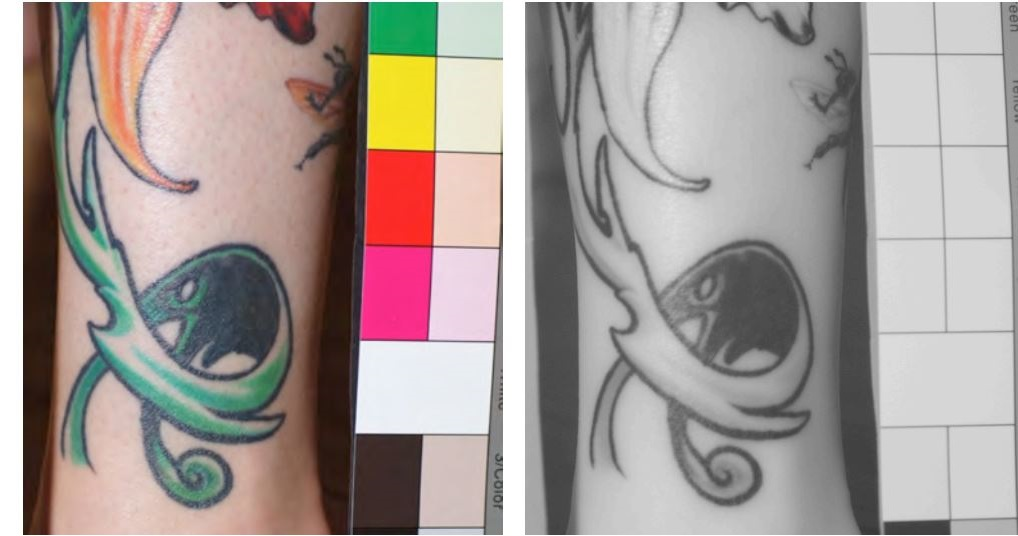
\includegraphics[scale=0.6]{figures/tattoo1.JPG}

\caption[Density comparison between a visible light image and an NIR one of a tattooed skin]{Density comparison between a visible light image and an NIR one of a tattooed skin. Low density regions in some colours like green, red and orange are partly invisible in the NIR image. Regions where green is mixed with black are visible.}\label{fig:tattoo1}
\end{figure}

\subsubsection{Dye Colour}
Ink colour is even more important than density, as some colours absorb more NIR light than others and a very thin layer of pigments can absorb most of the projected NIR light and, thus, prevent it to reach to the underlying veins. In \autoref{fig:tattoo2} \parencite{tatto},  dye density in the visible range is clearly intense. However, in the NIR range, tattoo is totally invisible because the used colours (red, yellow and orange) don’t absorb NIR light. Merely traces of the tattoo shape are visible in the NIR range. This is caused by the depigmentation of the underlying skin following healing of the skin after the tattoo \parencite{tatto} and has nothing to do with the tattoo itself or its colours.

\begin{figure}[H]
\centering
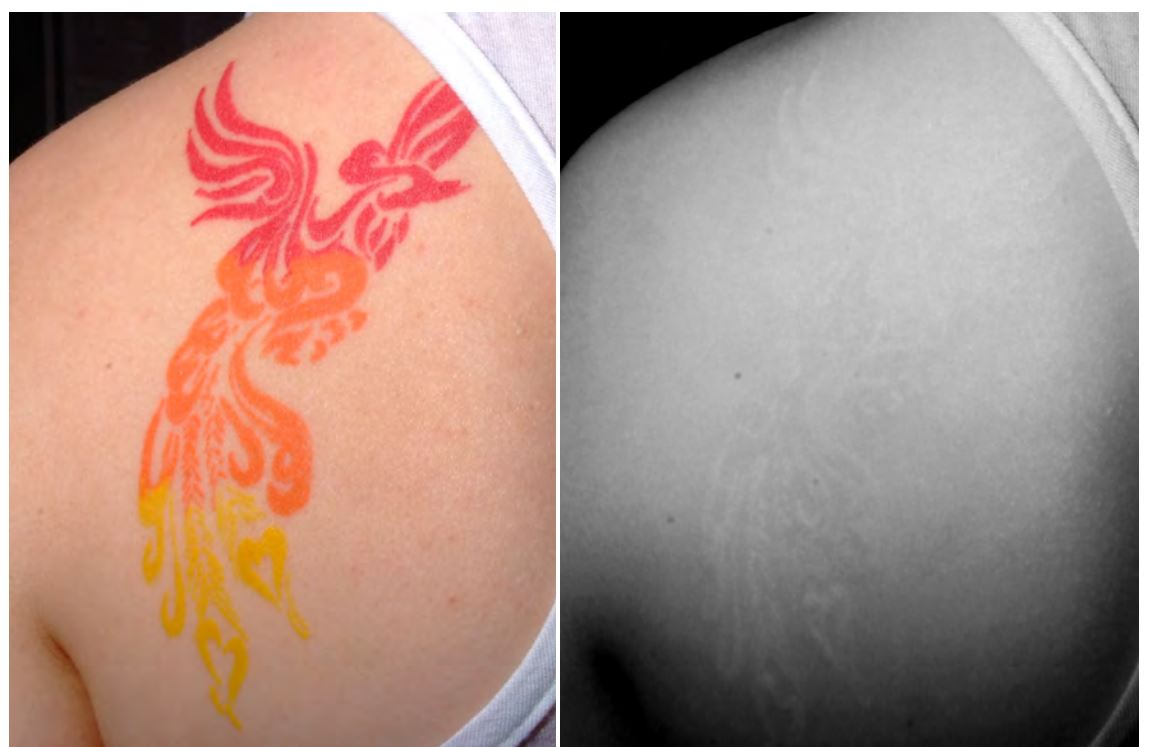
\includegraphics[scale=0.6]{figures/tattoo2.JPG}
\caption[Colour comparison between a visible light image and an NIR one of a tattooed skin]{Colour comparison between a visible light image and an NIR one of a tattooed skin.  }\label{fig:tattoo2}
\end{figure}


\subsubsection{Conclusion}

Tattoos can limit the visual examination of the veins when intense. NIR imaging can sometimes penetrate the tattoo pigments and let the operators see through them. Depending on the ink colour and intensity, NIR light can either be absorbed directly in the dermis by the tattoo pigments and behave just like the visible light or penetrate them to get absorbed then by the haemoglobin in the veins and results in good visualization of the veins. The \autoref{table:tattoo} \parencite{tatto} shows a brief summary of the effects of ink colour and density on the success of NIR visualization on a tattooed skin.


\begin{table}[H]
\setlength\extrarowheight{7pt}
\begin{tabular}{ | p{0.2\linewidth} | p{0.3\linewidth}| p{0.41\linewidth} |}
Property&Successful visualization&Unsuccessful visualization\\ \hline
Dye colour&Yellow, red, green, blue and light purple&Black and dark purple\\ \hline
Dye density& Light and pale tattoos & Colour	inks mixed with black.	The more black the less visible. \\ \hline
\end{tabular}
\captionof{table}{Effect of dye colour and density on the success of NIR imaging on a tattooed skin} \label{table:tattoo} 
\end{table}

\subsection{Results on Different Skin Colours} 

Skin colour plays a role in the NIR light visualization skin. The element that gives the skin its colour is melanin. The more melanin in the skin, the darker it is. As stated in the first chapter, absorption of epidermis in the NIR spectral range is defined almost exclusively by its melanin. That means, theoretically, darker skin types absorb more NIR light and, therefore, less light is transmitted to the dermis and the veins. 


\subsubsection{Fitzpatrick Skin Phototype}

The Fitzpatrick skin phototype classifies the skin types into six levels, shown in \autoref{table:fitzpatrick}, depending on the amount of melanin pigment in the skin. The melanin amounts determine the skin colour as well as the likelihood of burning.

\begin{table}[H]
\setlength\extrarowheight{7pt}
\begin{tabular}{ | p{0.2\linewidth} | p{0.3\linewidth}| p{0.41\linewidth} |}
Skin Type&Colour&Description\\ \hline
Type I&Pale white skin&Extremely sensitive skin, always burns, never tans\\ \hline
Type II& White skin&Very sensitive skin, burns easily, tans minimally\\ \hline
Type III&Light brown skin&Sensitive skin, sometimes burns, slowly tans to light brown\\ \hline
Type IV&Moderate brown skin&Mildly sensitive, burns minimally, always tans to moderate brown\\ \hline
Type V&Dark brown skin&Resistant skin, rarely burns, tans well\\ \hline
Type VI&Deeply pigmented dark brown to black skin&Very resistant skin, never burns, deeply pigmented\\ \hline
\end{tabular}
\captionof{table}{The Fitzpatrick skin phototype} \label{table:fitzpatrick} 
\end{table}

\subsubsection{Melanin Rate Effect}
Melanin can affect the NIR imaging indeed, but the difference in melanin rates between different human skin colours doesn’t play a major role in light absorption and scattering properties in the NIR range \parencite{skinTypes}. 

\subsubsection{Conclusion}
Despite the high melanin rate in darker skins, skin colour doesn’t limit the NIR vein visualization. A quick comparison between the results on skin of type VI and another of type II is performed. Both persons participated in this comparison are males and have close age and body weight.
The \autoref{fig:compare10} shows a row NIR image as well as the result after applying adaptive thresholding on a skin of type VI. Veins are good visualized in both images despite the high melanin rate. \autoref{fig:compare10} also shows two images in the same setting as in \autoref{fig:compare10}, but the skin type is II, which is brighter than the type VI.





\begin{figure}[H]
\centering
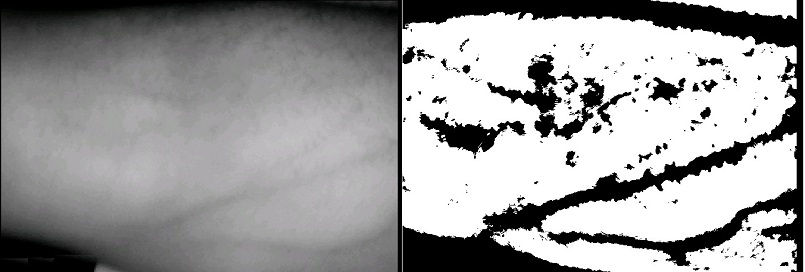
\includegraphics[scale=0.8]{figures/compare10.jpg}
\caption[Row NIR image and the result of adaptive thresholding on a skin of type VI]{Row NIR image and the result of adaptive thresholding on a skin of type VI. Veins are good visualized despite the high melanin rate.}\label{fig:compare10}
\end{figure}

\begin{figure}[H]
\centering
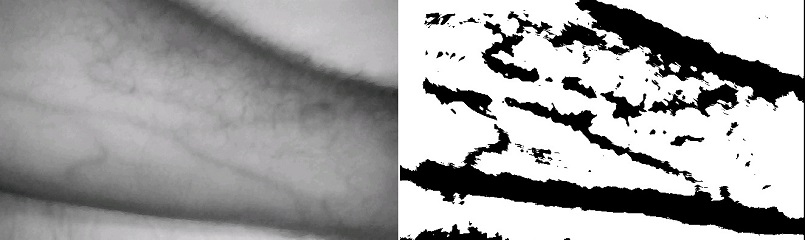
\includegraphics[scale=0.8]{figures/compare11.JPG}
\caption[Row NIR image and the result of adaptive thresholding on a skin of type II]{Row NIR image and the result of adaptive thresholding on a skin of type II. Veins are good visualized.}\label{fig:compare11}
\end{figure}

\subsection{Results on Skin with Diseases}

Although most of skin diseases don’t limit the venepuncture procedure, some skin diseases can be a real suffering for patients. It is sometimes near to impossible to locate the vein just by visual examination and palpation.

\subsubsection{Scleroderma}
Scleroderma is a chronic autoimmune disorder characterized by the hardening of connective tissue, internally and externally. The initial symptom for both forms is usually the hardening and tightening of the skin. In its advanced stages, skin, and skin of the arms, can be as hard as the skin on the heels. 

\subsubsection{Scleroderma: Clinical Study}
We performed a study on a 56 years old female patient with advanced scleroderma. Regular clinical treatments of this disease often require an intravenous access. However, obtaining this access is near to impossible without any imaging devices. The \autoref{fig:maVis} shows a visible range image of her arm. No veins can be located visually in the image and a needle mark of a failed venepuncture attempt is visible. 3-5 failed attempts to obtain the intravenous access have been recorded each time a clinical treatment is required. Important treatments have been cancelled because operators and even doctors at university hospitals were unable to perform the venepuncture operation. The suggested solution was to implant a permanent device. A port in the chest that is connected directly to the heart. This implantation operation is usually recommended to scleroderma patients in middle to advanced stages.


\begin{figure}[H]
\centering
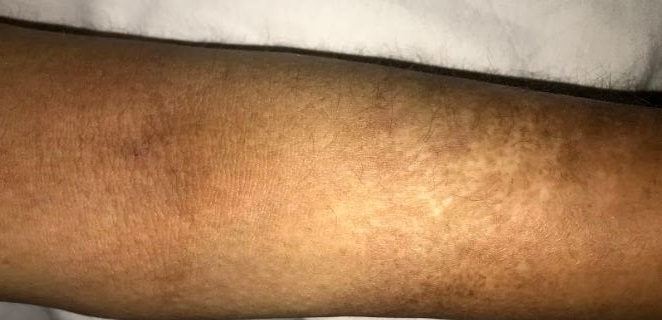
\includegraphics[scale=0.8]{figures/maVis.JPG}
\caption[Visible range image of a scleroderma patient arm skin]{Visible range image of a scleroderma patient arm skin. Skin is extremely hardened. Veins cannot be located visually.}\label{fig:maVis}
\end{figure}


\subsubsection{Scleroderma: Ultrasound Vein Imaging}
Practically, using ultrasound imaging with colour Doppler has increased the venepuncture success rate to 100\%.
Nevertheless, as mentioned in the first chapter, it requires well understanding of the Doppler image generation, high hand-eye-coordination skill and, of course, the availability of the device itself. 


\subsubsection{Scleroderma: Results}
The \autoref{fig:compare12} shows results of the proposed solution on the arm of the given scleroderma patient. Veins can be seen in the raw NIR image, but they appear to be clearer and with more contrast in the processed one.
\begin{figure}[H]
\centering
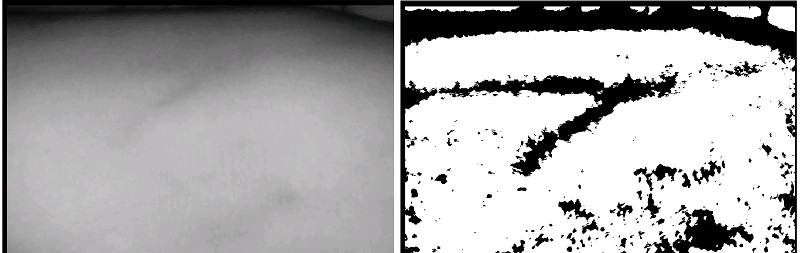
\includegraphics[scale=0.8]{figures/compare12.JPG}
\caption[NIR image and the result of applying adaptive thresholding on a scleroderma patient's arm]{NIR image and the result of applying adaptive thresholding on a scleroderma patient's arm. Veins are visualized.}\label{fig:compare12}
\end{figure}

\section{Conclusion}

In their different forms, medical imaging techniques have become an essential part of any clinical operation. Peripheral veins imaging technologies are gradually getting more attention and investment, but they are expensive, and their availability is limited to very special clinics. We proposed a low-cost mobile vein viewing system, utilizing near infrared light and a simple digital camera. The focus is to develop a viewing system of the pattern of peripheral veins, but optimized to make the venepuncture operation easier. The prototype has shown promising results in terms of vein visualization and ease-of-use on different skin types and conditions.

\section{Future Work and Possible Application Areas}
Further research in mobile vein viewing approaches can go in many different directions such as machine learning or using another technology such as Ultrasound. Applications for the proposed solution can take place also in many different areas related to vein imaging.

\subsection{Hybrid Technology, NIR + US}
Ultrasound imaging devices has become more mobile and cheaper. Initially, at the begging of this work, we faced the decision of using either NIR or US imaging. We chose NIR due to their high availability, low cost and ease-of-use. US imaging, as stated earlier, has many features such as vein depth estimation. But using US devices in this field, however, is limited because of their big size and high cost. Luckily, since 2009, researchers at Washington University have developed a line of low-cost ultrasound probes that run on small PCs and mobile devices. 


A hybrid method that utilizes both NIR and US technologies using a smartphone can be a good candidate for further research. Automatic comparison between the NIR and US images can provide information about vein location, depth and status. The software has to understand and analyse both images to extract such information.


\subsection{Burns Assessment}

Evaluation of the surface and the depth of skin burn is essential, as such evaluation enables the appropriate choice of treatment. Clinical assessment is currently the most frequently applied method in burn depth evaluation. It is, however, error-prone and not accurate. Using NIR imaging can provide more information about the burn severity and depth \parencite{burn}.

\subsection{Skin Abnormalities Recognition}

Many skin abnormalities can be examined visually, however, some diseases, like cancer, are hard to be detected visually. Skin cancer is the most common human cancer. The clinical diagnosis is often difficult as many benign skin lesions resemble malignancies upon visual examination, thus analysis of skin biopsies remains the standard diagnosis. A rapid, non-invasive technique that could be utilized for characterization of skin lesions prior to biopsy would be useful \parencite{skinCancer}.
LEDs with different wavelengths can be utilized and controlled through a control circuit. Application then measures and compares different records in different wavelengths.

